Android Studio kan als IDE zelf nieuwe projecten aanmaken met \textit{File > New > New Project\dots}. 
Hierna wordt een overzicht getoond van projecten die als basis kunnen worden gebruikt. Ook 
kan er op dit scherm gekozen worden voor welk apparaat de applicatie is.
\begin{figure}[H]
    \centering
    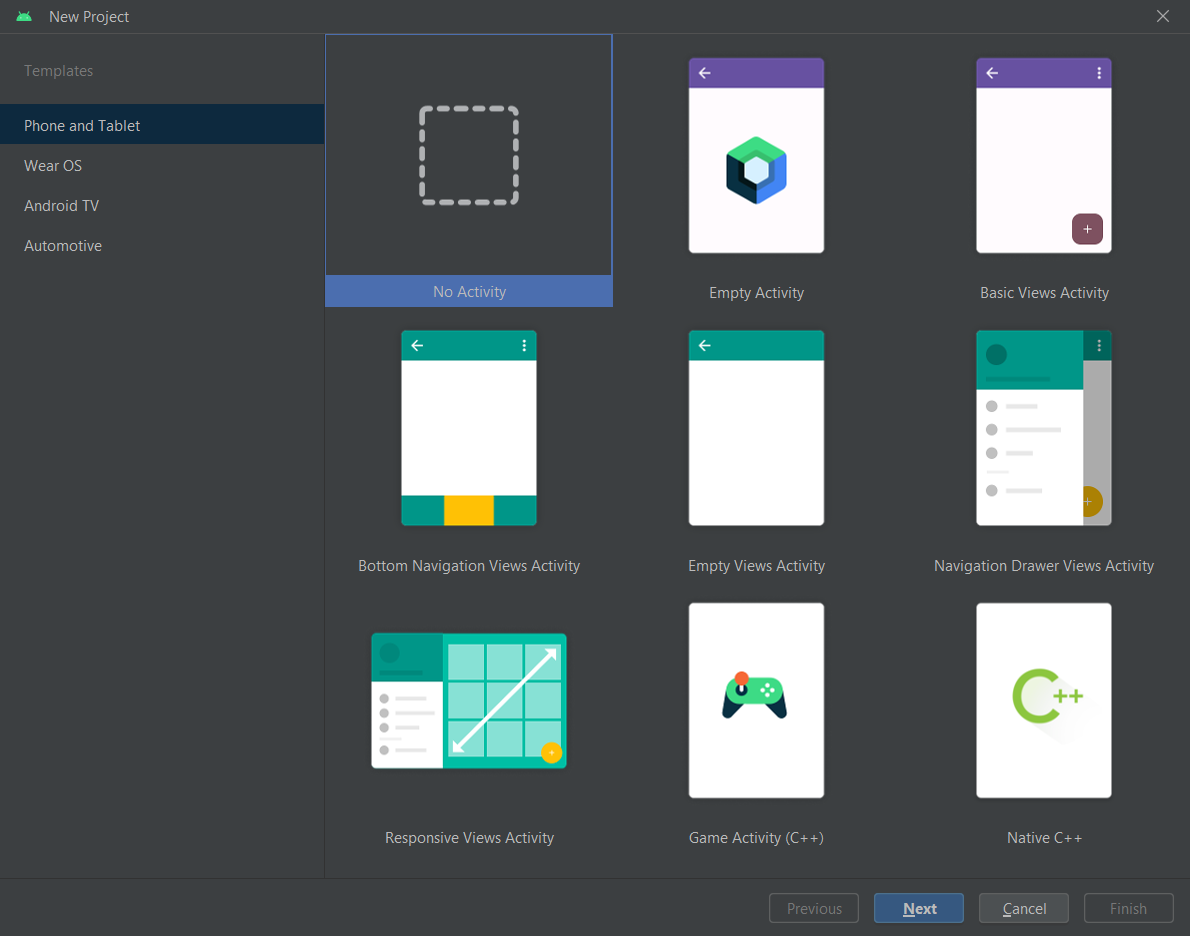
\includegraphics[height=0.35\textheight]{OverzichtProjecten.png}
    \caption{Overzicht startprojecten Android Studio.}
\end{figure}
Afhankelijk van de functionaliteit die wordt geïmplementeerd, zal een ander 
startproject gekozen worden. Na het kiezen van het startproject kan een naam, 
programmeertaal en de minimaal ondersteunde Android API worden ingegeven. Voor dit onderzoek wordt er gekozen 
voor Kotlin. De naam en minimale ondersteunde Android API spelen hierbij geen rol.

\subsection{Basisfunctionaliteiten}
\label{par:basisfunctionaliteiten}
Bij de basisfunctionaliteiten wordt
\textbf{Bottom Navigation Views Activity} als startproject gebruikt om te kunnen navigeren tussen 
verschillende schermen. Daardoor moeten er geen extra libraries worden geïmplementeerd.

\subsection{Overige functionaliteiten}
Voor de overige functionaliteiten (gebruik van sensoren, 
push-notificaties en audio- en videospelers) wordt
\textbf{Empty Views Activity} als startproject gebruikt. Op die manier zal er zo weinig mogelijk 
\gls{overhead} zijn die de resultaten kan beïnvloeden.

\subsection{Firebase Performance Monitoring}
Om de performantie van de applicaties te meten, meer specifiek de tijdsduur 
die een stuk code nodig heeft om uit te voeren, 
wordt de Firebase Performance Monitoring tool in het project geïmplementeerd. 

\paragraph{Firebase aan project toevoegen}
Vooraleer de Performance Monitoring tool geïmplementeerd kan worden, moet Firebase 
aan het project worden toegevoegd.

\subparagraph{1. Configuratie bestanden toevoegen}
In het Firebase project voegen we een nieuwe Android applicatie toe. Om deze aan te maken geven we de package naam 
dat te vinden is in build.gradle(module) bestand als applicationId en optioneel de naam van de applicatie mee.
\\\\
Na dat de Android applicatie is aangemaakt, moeten we het \textbf{google-services.json} bestand downloaden. 
Deze plaatsen we dan in de \textit{app} folder.

\subparagraph{2. Firebase plugins configureren}
Om Firebase het configuratiebestand nu te laten gebruiken moeten we de google-services plugin toevoegen aan 
de dependancies in het build.gradle(project) bestand boven de plugins. 
\begin{minted}{java}
buildscript {
    repositories {
        google()
        mavenCentral()
    }

    dependencies {
        // andere dependancies
        classpath "com.google.gms:google-services:4.3.15"
    }
}
\end{minted}
Daarna moeten we de plugin uitvoeren door deze aan het build.gradle(module) bestand toe te voegen.
\begin{minted}{java}
plugins {
    // andere plugins 
    id "com.google.gms.google-services"
}
\end{minted}
Tot slot moeten we de Firebase SDKs toevoegen aan het build.gradle(module) bestand.
\begin{minted}{java}
dependencies {
    // andere dependancies
    implementation platform("com.google.firebase:firebase-bom:32.0.0")
}
\end{minted}
Firebase is nu volledig aan ons project toegevoegd.

\paragraph{Implementatie Performance Monitoring tool}
Nu Firebase aan ons project is toegevoegd, kan de Performance Monitor 
worden toegevoegd.

\subparagraph{1. Performance Monitoring SDK aan applicatie toevoegen}
Als eerst voegen we de Performance Monitor SDK toe aan ons project in het \textbf{build.gradle(module)} bestand.
\begin{minted}{java}
dependencies {
    // ... andere dependancies
    implementation "com.google.firebase:firebase-perf-ktx"
}
\end{minted}

\subparagraph{2. Performance Monitoring Gradle plugin toevoegen}
Na het toevoegen van de SDK moeten we de Perormance Monitoring Gradle plugin toevoegen. 
Dit doen we door de dependancies hiervan toe te voegen aan het \textbf{build.gradle(project)} bestand.
\begin{minted}{java}
dependencies {
    // ... andere dependancies
    classpath "com.google.firebase:perf-plugin:1.4.2"
}
\end{minted}
Tot slot voegen we de plugin toe. Dit doen we door deze in het \textbf{build.gradle(module)} bestand toe te voegen.
\begin{minted}{java}
plugins {
    // ... andere plugins
    id "com.google.firebase.firebase-perf"
}
\end{minted}
Nu is het blanco project klaar om vanuit dit project alle functionaliteiten te 
implementeren en onderzoeken, buiten de basisfunctionaliteiten. Hiervoor zullen we vanuit een ander project starten, 
maar zullen we de Perormance Monitoring tool op dezelfde manier implementeren.

\subparagraph{3. Performance meten}
Nu kunnen we een trace maken om de performantie te meten. Doorheen de applicaties zal dit er als 
volgt uitzien.
\begin{minted}{java}
val trace = FirebasePerformance.getInstance().newTrace("naam_trace")

trace.start()
// uit te voeren code
trace.stop()
\end{minted}
De trace wordt gestart voor de code die we willen meten en gestopt na de code die we willen meten.
De trace wordt dan automatisch naar de Firebase console gestuurd. Hier kunnen we de trace terugvinden
en de performantie analyseren.
